\section*{Introduction}

\addtocounter{chapter}{1}
\setcounter{figure}{0}

In the third\todo{was ``second'', changed to ``third''} part of this book, I will study the self-organisation of
language systems that are based on a single strategy. In order to do
so, I need to introduce the adoption, alignment and invention
operators for that strategy. The \textsc{adoption operator}\is{adoption operator|see{learning operators}}\is{learning operators} specifies how language users can pick up items of the language
system. The \textsc{alignment operator}
\is{alignment operator|see{learning operators}}
specifies how agents should
update their linguistic knowledge after a communicative
interaction. The \textsc{invention operator}
\is{invention operator|see{learning operators}}
is triggered when the
(current knowledge of) the language system is insufficient or when the
current language system is considered to be inefficient
\citep{steels06how}.

The performance of the adoption and the alignment operator can be
evaluated in an \textsc{acquisition experiment}\is{acquisition experiment} 
in which one agent
acquires a predefined language system through playing language games.
This evaluation is achieved by comparing the communicative success of the
learner to the communicative success of two agents that share the
predefined language system. The predefined language systems are
implemented as in the baseline experiments in Part
\ref{s:language-strats}.

The invention operator can be evaluated in a \textsc{formation
  experiment}\is{formation experiment} in which a population of
agents needs to construct its own language system based on one
language strategy and allows agents to extend the current language
system. These innovations can be picked up by other agents using the
adoption operators. After each interaction agents align their
knowledge of the language system using the alignment operator. This
alignment operator allows agents to track their (local view on) the
communicative success of certain linguistic items, which they can use
to prefer one linguistic item over the other. At the system level this
mechanism can lead to the dominance of one item over the other and to
the disappearance of items that are disused. The complete process of
how a language strategy can construct a language system is illustrated
in \figref{f:strategies-1}.\enlargethispage{3\baselineskip}

\begin{figure}
  \begin{center}
    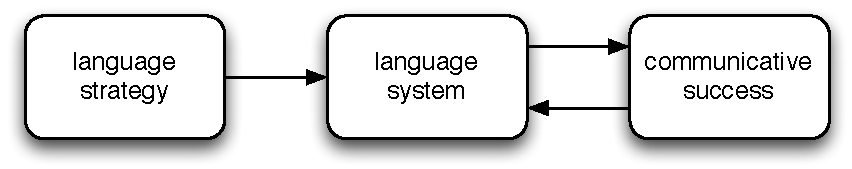
\includegraphics[width=0.7\textwidth]{./intro/figures/strategies-1.pdf}
    \caption[The construction of a language system based on a single
    language strategy]{The construction of a language system based on
      a single language strategy. The language strategy allows agents
      to expand the language system. Based on a feedback loop which
      reflects success in communication, an agent can prefer linguistic
      items that are more successful, whereas unsuccessful linguistic items
      can be removed from the language system.}
    \label{f:strategies-1}
  \end{center}
\end{figure}

\addtocounter{chapter}{-1}

\thispagestyle{empty}








